\documentclass{amsart}

\newcommand{\cA}{\mathcal{A}}\newcommand{\cB}{\mathcal{B}}
\newcommand{\cC}{\mathcal{C}}\newcommand{\cD}{\mathcal{D}}
\newcommand{\cE}{\mathcal{E}}\newcommand{\cF}{\mathcal{F}}
\newcommand{\cG}{\mathcal{G}}\newcommand{\cH}{\mathcal{H}}
\newcommand{\cI}{\mathcal{I}}\newcommand{\cJ}{\mathcal{J}}
\newcommand{\cK}{\mathcal{K}}\newcommand{\cL}{\mathcal{L}}
\newcommand{\cM}{\mathcal{M}}\newcommand{\cN}{\mathcal{N}}
\newcommand{\cO}{\mathcal{O}}\newcommand{\cP}{\mathcal{P}}
\newcommand{\cQ}{\mathcal{Q}}\newcommand{\cR}{\mathcal{R}}
\newcommand{\cS}{\mathcal{S}}\newcommand{\cT}{\mathcal{T}}
\newcommand{\cU}{\mathcal{U}}\newcommand{\cV}{\mathcal{V}}
\newcommand{\cW}{\mathcal{W}}\newcommand{\cX}{\mathcal{X}}
\newcommand{\cY}{\mathcal{Y}}\newcommand{\cZ}{\mathcal{Z}}


\newcommand{\bA}{\mathbb{A}}\newcommand{\bB}{\mathbb{B}}
\newcommand{\bC}{\mathbb{C}}\newcommand{\bD}{\mathbb{D}}
\newcommand{\bE}{\mathbb{E}}\newcommand{\bF}{\mathbb{F}}
\newcommand{\bG}{\mathbb{G}}\newcommand{\bH}{\mathbb{H}}
\newcommand{\bI}{\mathbb{I}}\newcommand{\bJ}{\mathbb{J}}
\newcommand{\bK}{\mathbb{K}}\newcommand{\bL}{\mathbb{L}}
\newcommand{\bM}{\mathbb{M}}\newcommand{\bN}{\mathbb{N}}
\newcommand{\bO}{\mathbb{O}}\newcommand{\bP}{\mathbb{P}}
\newcommand{\bQ}{\mathbb{Q}}\newcommand{\bR}{\mathbb{R}}
\newcommand{\bS}{\mathbb{S}}\newcommand{\bT}{\mathbb{T}}
\newcommand{\bU}{\mathbb{U}}\newcommand{\bV}{\mathbb{V}}
\newcommand{\bW}{\mathbb{W}}\newcommand{\bX}{\mathbb{X}}
\newcommand{\bY}{\mathbb{Y}}\newcommand{\bZ}{\mathbb{Z}}

\newcommand{\id}{\text{id}}\newcommand{\C}{\mathbb{C}}
\newcommand{\Z}{\mathbb{Z}}


\usepackage{lmodern, listings}
\usepackage[dvipsnames,svgnames,x11names,hyperref]{xcolor}
\usepackage{url,verbatim,amssymb,enumerate,stmaryrd,bbm,mathtools,microtype}
\usepackage[pagebackref,colorlinks,citecolor=Mahogany,linkcolor=Mahogany,urlcolor=Mahogany,filecolor=Mahogany]{hyperref}
\usepackage{setspace}
\setstretch{1.08}

\usepackage{tikz,tikz-cd}
\usetikzlibrary{matrix,calc,positioning,arrows,decorations.pathreplacing,patterns,knots}

% tikz regular polygons
\newdimen\R
\R=1.5cm


\newtheorem{theorem}{Theorem}[section]
\newtheorem{lemma}[theorem]{Lemma}
\newtheorem{proposition}[theorem]{Proposition}
\newtheorem{corollary}[theorem]{Corollary}
\newtheorem*{corollary*}{Corollary}
\newtheorem{conjecture}[theorem]{Conjecture}
\newtheorem{metatheorem}[theorem]{Meta-theorem}
\newtheorem{theoreminprogress}[theorem]{Theorem-in-progress}
\theoremstyle{definition}
\newtheorem{notation}[theorem]{Notation}
\newtheorem{convention}[theorem]{Convention}
\newtheorem{definition}[theorem]{Definition}
\newtheorem*{problem}{Problem}
\theoremstyle{remark}
\newtheorem{example}[theorem]{Example}
\newtheorem{remark}[theorem]{Remark}
\newtheorem{warning}[theorem]{Warning}
\newtheorem{question}[theorem]{Question}
\newtheorem{discussion}[theorem]{Discussion}

%TODO NOTES
\usepackage{xargs}                      % Use more than one optional parameter in a new commands
% 
\usepackage{xcolor}
\usepackage[colorinlistoftodos,prependcaption,textsize=tiny]{todonotes}
\newcommandx{\note}[2][1=]{\todo[linecolor=red,backgroundcolor=red!25,bordercolor=red,#1]{#2}}


\usepackage{wrapfig,caption}
\captionsetup{
	font=small}

\newcommand{\cat}[1]{\mathsf{#1}}
\newcommand{\mr}[1]{{\rm #1}}

\renewcommand\labelitemi{{\boldmath$\cdot$}}

\usepackage{graphicx}
\graphicspath{{./figures/}}

\title[CS283 Final Project]{Fisherfaces Under Simulated Perspective Distortions}
\author{Natalia Pacheco-Tallaj and Toby Satterthwaite\\
\today }

% \date{\today}


\begin{document}

\maketitle
\section{Introduction}
P.Belhumeur, et al.'s 1997 paper \textit{Eigenfaces vs. Fisherfaces: Recognition Using Class-Specific Linear Projection} proposes an improvement upon previous face-recognition algorithms to better account for variation in photos of the same person in a data set. They consider images as column vectors $\vec{x}_1,\ldots, \vec{x}_N$ in a high-dimensional space $\bR^n$ (where $n$ is dependent on number of pixels). The previous face-recognition method that the paper improves upon, called Eigenfaces, uses principal component analysis (PCA) to map the $\vec{x}_k$ to lower-dimensional \textit{feature vectors} $\vec{y}_k = W^T\vec{x}_k$ such that the scatter of the feature vectors is maximized:
\begin{equation}
    W_{pca} = \text{arg}\max_W |W^T S_T W|
    \label{eq:pcaintro}
\end{equation}
where $S_T$ is the total scatter matrix of the $\vec{x}_k$, $S_T = \sum_{i=1}^N (\vec{x}_k - \vec{\mu}) (\vec{x}_k - \vec{\mu})^T$, where $\vec{\mu}$ is the image mean. 

Usually images are divided into a number of classes $X_1, \ldots, X_c$ (in the case of face recognition, each class is a different person). The issue with Eigenfaces is that by maximizing a total scatter function, it is not only maximizing scatter between image classes but also within image classes. This is particularly harmful if we are working with datasets with variation in lighting conditions within each class, because the Eigenfaces (principal components) retain this variation information. The paper proposes a solution, called Fisherfaces, using the Fisher linear discriminant (FLD) method to extract the feature vectors, which seeks to solve the problem of maximizing between-class scatter of the projected feature vectors $\vec{y}_k$ while minimizing within-class scatter:
\begin{equation}
    W_{fld} = \text{arg}\max\limits_W \frac{|W^T S_B W|}{|W^TS_WW|}
    \label{eq:fldintro}
\end{equation}
where $S_W$ is the within-class scatter matrix and $S_B$ the between-class scatter matrix of the $\vec{x}_k$:$S_W = \sum_{i=1}^c N_i (\vec{\mu}_i-\vec{\mu})(\vec{\mu}_i -\vec{\mu})^T$ and $S_B &= \sum_{i=1}^c\sum_{\vec{x}_k\in X_i}(\vec{x}_k-\vec{\mu}_i)(\vec{x}_k - \vec{\mu}_i)^T$, where $\vec{\mu}_i$ is the $i$-th class's mean and $N_i$ the number of images in class $i$.

The authors test the performance of their algorithm against variation in lighting and facial expression, but does not test for other important variation in facial recognition applications such as perspective distortion. Our goal is to test how the Fisherfaces algorithm proposed in the paper fares against different kinds of increasingly drastic perspective distortion. We apply different kinds of affine transformations with increasing deviation from the identity to our test images and quantify the loss of accuracy with these perspective distortions.

% Let $\vec{x}_1,\ldots, \vec{x}_N$ be vectorized images, each a column vector of length $n$. They belong to $c$ classes $X_1,\ldots, X_c$. The Eigenfaces method for face recognition was based on solving a single scatter matrix problem: compute new feature vectors $\vec{y}_k = W^T\vec{x}_k$ of lower dimension by taking $W\in \R^{n\times m}, m < n$ to be 
% $$W_{opt} = \text{arg}\max_W |W^T S_T W| = \begin{pmatrix}\vec{w}_1&\ldots&\vec{w}_m\end{pmatrix}$$
% where $\vec{w}_i$ are the $n$-dimensional eigenvectors of $S_T$ corresponding to the $m$ largest eigenvalues, and $S_T$ is the total scatter matrix of all vectorized images
% $$S_T = \sum_{i=1}^N (\vec{x}_k - \vec{\mu}) (\vec{x}_k - \vec{\mu})^T$$
% and $\vec{\mu}$ is the mean of all $\vec{x}_k$.  The $\vec{w}_i$ are referred to as the Eigenfaces, and this method of dimensionality reduction is known as principal component analysis (PCA). The issue with Eigenfaces is that by maximizing a total scatter function, it is not only maximizing scatter between image classes but also within image classes. This is particularly harmful if we are working with datasets with variation in lighting conditions within each class, because the Eigenfaces (principal components) retain this variation information. 

% However the paper proposes an improvement upon this method called Fisherfaces, where this issue is corrected by instead maximizing between-class scatter while at the same time minimizing within-class scatter. 
% $$W_{opt} = \text{arg}\max\limits_W \frac{|W^T S_B W|}{|W^TS_WW|} = \begin{pmatrix}\vec{w}_1 &\ldots & \vec{w}_m\end{pmatrix} $$
% where $w_i$ are the generalized eigenvectors for the $m$ largest generalized eigenvalues $\lambda_i$:
% $$S_B \vec{w}_i = \lambda_iS_W\vec{w}_i$$
% this type of dimensionality reduction is called the Fisher Linear Discriminant method (FLD). 

% To solve {\color{red}some issue with some matrix being singular}, this should be implemented in two stages, first a PCA stage and then an FLD stage:
% $$W_{opt} = W_{pca}W_{fld} $$ 
% Tha peper solves 
% \begin{align*}
% 	W_{pca} &= \text{arg}\max\limits_W|W^TS_TW|\\
% 	W_{fld} &= \text{arg}\max\limits_W\frac{|W^TW_{pca}^TS_BW_{pca}W|}{|W^TW_{pca}^TS_WW_{pca}W|}
% \end{align*}
% Solving this two step problem is the same as solving FLD, since $\frac{|W_{fld}^TW_{pca}^TS_BW_{pca}W_{fld}|}{|W_{fld}^TW_{pca}^TS_WW_{pca}W_{fld}|} = \frac{|W^T S_B W|}{|W^TS_WW|}$. 


\section{Methods}
In face recognition applications, there is a problem with solving Equation~\ref{eq:fldintro} directly: the rank of $S_W$ is bounded above by the number of $N$ images in the training set, much smaller than the length $n$ of the image vectors which determines the size $n\times n$ of $S_W$. Then $S_W$ is singular and $|W^TS_WW|$ can be exactly $0$. To solve this issue, we must first reduce the dimensions of the data set with PCA so that it equals the number of data points, and then apply FLD to the reduced dataset: 
\begin{align*}
	W_{pca} &= \text{arg}\max\limits_W|W^TS_TW|\\
	W_{fld} &= \text{arg}\max\limits_W\frac{|W^TW_{pca}^TS_BW_{pca}W|}{|W^TW_{pca}^TS_WW_{pca}W|}
\end{align*}
Computing scatter matrices is very expensive. With our dataset, images of about $300,000$ pixels each would yield $300,000\times 300,000$ scatter matrices (or about $90$ gigabytes). However, we can avoid computing any of the scatter matrices by using SVD to find the dimension-reduced feature vectors. Below we show how to perform the PCA and FLD steps of the paper's Fisherfaces algorithm using SVD. 

\subsection{PCA step with SVD}
The problem
\begin{equation*}W_{pca} = \text{arg}\max_W |W^T S_T W|
\label{eq:pca}\end{equation*}
is solved by the matrix 
$W = \begin{pmatrix} \vec{w}_1 & \ldots & \vec{w}_m\end{pmatrix} $
where $\vec{w}_k$ are the $m$ eigenvectors corresponding to the $m$ largest eigenvalues of $S_T$. 
We can express $S_T$ as $X^TX$ where 
$$X = \begin{pmatrix}\vec{x}_1^T\\ \vdots \\ \vec{x}_N^T\end{pmatrix} - \begin{pmatrix} \vec{\mu}^T\\ \vdots \\\vec{\mu}^T\end{pmatrix} $$
is the matrix with the vectorized images minus the mean image as its rows. 
% Then 
% $$S_T = X^T X $$
% and therefore $S_T^T = S_T$, i.e. $S_T$ is symmetric. It can thus be diagonalized. In fact, if we let $A = \begin{pmatrix} \vec{w}_1 & \ldots & \vec{w}_k\end{pmatrix}$ where each $\vec{w}_k$ is an eigenvector of $S_T$, ordered by decreasing order of their eigenvalues, then for the standard basis vector $\vec{e}_i$, 
% $A^{-1}S_T A e_i = A^{-1}S_T \vec{w}_i = A^{-1}\lambda_i\vec{w}_i = \lambda_i A^{-1} \vec{w}_i = \lambda_i \vec{e}_i$, so 
% $$A^{-1}S_T A = \begin{pmatrix} \lambda_1 & 0  & \ldots \\ 0 & \lambda_2 & \ldots \\ \vdots & \vdots & \ddots \end{pmatrix} = D_T$$
% where $\lambda_1, \ldots$ are the eigenvalues ordered in decreasing order.
Now if we take the SVD of $X$ we get $X = UDV^T$ with $S$ the diagonal matrix of singular values of $X$ in decreasing order. The singular values of $X$ are by definition the square roots of the 
% TODO: nonnegative eigenvalues tho
eigenvalues of $X^TX = S_T$, so $D^2$ is the matrix of eigenvalues of $S_T$. Therefore: 
$$S_T = X^T X = VDU^TUDV^T = VD^2V^T = VD_TV^{-1} $$
($U, V$ are unitary) so $S_TV = VD_T$, then the columns of $V$ are the eigenvectors. Thus the first $m$ columns of $V$ give us the solution to \ref{eq:pcaintro}, and the feature vectord $y_k$ are then the rows of $XV$. 
% In PCA, the feature vectors $\vec{y}_k$ are obtained by truncating $V$ to the $m$-th column, call the result $W$, and then applying the transpose to $\vec{x}_k$. Thus $y_k$ are the columns of $W^T X^T$, or equivalently the rows of $XW$. 
If we set $m = N$ to be the amount of images, we can do this with numpy by taking 
\begin{lstlisting}
	_, _, vh = np.linalg.svd(X, full_matrices=False)
	W = vh.transpose()

	# the rows of Y are the feature vectors, 
	# there are N such vectors of length N each
	Y = np.dot(X, V)
\end{lstlisting}

\subsection{FLD with SVD}
% Ok, so that's SVD for Eigenfaces involving a single scatter matrix. However, the Fisherfaces method that the paper proposes uses the Fished Linear Discriminant method involving two different scatter matrices. More precisely,
% $$W_{opt} = \text{arg}\max\limits_W \frac{|W^T S_B W|}{|W^TS_WW|} = \begin{pmatrix}\vec{w}_1 &\ldots & \vec{w}_m\end{pmatrix} $$
% where $w_i$ are the generalized eigenvectors for the $m$ largest generalized eigenvalues $\lambda_i$:
% $$S_B \vec{w}_i = \lambda_iS_W\vec{w}_i$$
% $$W_{opt} = W_{pca}W_{fld} $$ 
The problem
\begin{equation}W_{fld} = \text{arg}\max\limits_W \frac{W^T W_{pca}^TS_BW_{pca} W}{W^T W_{pca}^TS_WW_{pca} W}\label{eq:fld} \end{equation}
is solved by the matrix $W = \begin{pmatrix} \vec{w}_1 & \ldots & \vec{w}_m\end{pmatrix}$ where $\vec{w}_k$ are the generalized eigenvectors with largest generalized eigenvalues (they solve the equation $S_b \vec{w}_k = \lambda_k S_w\vec{w}_k$).
To replicate what we did in the previous part we want to express $W_{pca}^TS_B, W_{pca}^TS_WW_{pca}$ as some matrix times its transpose. Let 
$$M = \begin{pmatrix}\vec{\mu}_1^T \\ \vdots \\ \vec{\mu}_c^T\end{pmatrix} - \begin{pmatrix}\vec{\mu}^T \\ \vdots \\ \vec{\mu}^T\end{pmatrix} $$
then 
$$S_B = M^TM\text{ and } W_{pca}^TS_BW_{pca} = (MW_{pca})^T(MW_{pca}) $$
and let 
$$K = \begin{pmatrix} \vec{x}_1^T \\\vdots \\ \vec{x}_i^T\\\vec{x}_{i+1}^T\\\vdots \vec{x}_N^T\end{pmatrix} - \begin{pmatrix}\vec{\mu}_1^T \\\vdots\\\vec{\mu}_1^T\\\vec{\mu}_2^T\\\vdots\\\vec{\mu}_c^T\end{pmatrix} $$
where we are assuming the images are ordered by which class they belong to, then
$$S_W = K^TK \text{ and } W_{pca}^TS_WW_{pca} = (KW_{pca})^T(KW_{pca})$$
To simplify notation from now on we let $S_B, S_B$ denote $W_{pca}^TS_B, W_{pca}^TS_WW_{pca}$ and $M,K$ denote $MW_{pca}, KW_{pca}$. 
Here's the solution to the generalized eigenvalue problem without computing scatter matrices. \\
\textbf{Step 1. }Find $V_W$ that diagonalizes $S_W$ by taking the SVD $K = U_W D_W V_W^T$. By what we showed in section 1, $V_W^T S_W V_W = D_W^2$.\\
\textbf{Step 2. }Let 
\begin{align*}
	V_W' &= V_W D_W^{-1}\\ 
	M' &= MV_W'\\
	S_B' &= V'_W^TS_BV_W' = M'^TM'\\
\end{align*}
where $D_W^{-1}$ is obtained by inverting each element in the diagonal. Then $V_W'^T S_W V_W' = D_W^{-1}V_W^TS_WV_WD_W^{-1} = D_W^{-1} D_W^2 D_W^{-1} = I$. \\
\textbf{Step 3. }Find $V_B$ that diagonalizes $S_B'$ by taking the SVD $M' = U_B D_B V_B^T$, so that $V_B^TS_B' V_B = D_B^2$. \\
\textbf{Step 4. }Let $$V = V'_W V_B$$
We can then see that $V^TS_BV = V_B^TV_W'^T S_B V_W'V_B = V_B^TS_B'V_B = D_B^2$ and $V^TS_WV = V_B^TV_W'^T S_W V_W'V_B = V_B^TIV_B = I$, so 
$$S_BV = S_WVD_B^2$$
where $D_B$ is diagonal, from this equation we can see that the $i$-th column of $V$ is a generalized eigenvector with generalized eigenvalue the $i$-th diagonal entry of $D_B^2$. So the first $m$ columns of $V$ give us the solutions to \ref{eq:fldintro}.

\subsection{Data Set}

We test this approach on The Extended Yale Face Database B. This data set contains 28 human subjects who are each photographed in nine poses under 64 different lighting conditions for a total of 16128 images. For the purposes of running the simulation on a laptop computer, however, we limited ourselves to 15 classes (people) with 20 randomly selected samples per person for training and 15 randomly selected samples per person for testing.

\begin{figure}
\caption{One human subject in our data set under different expressions and lighting conditions.}
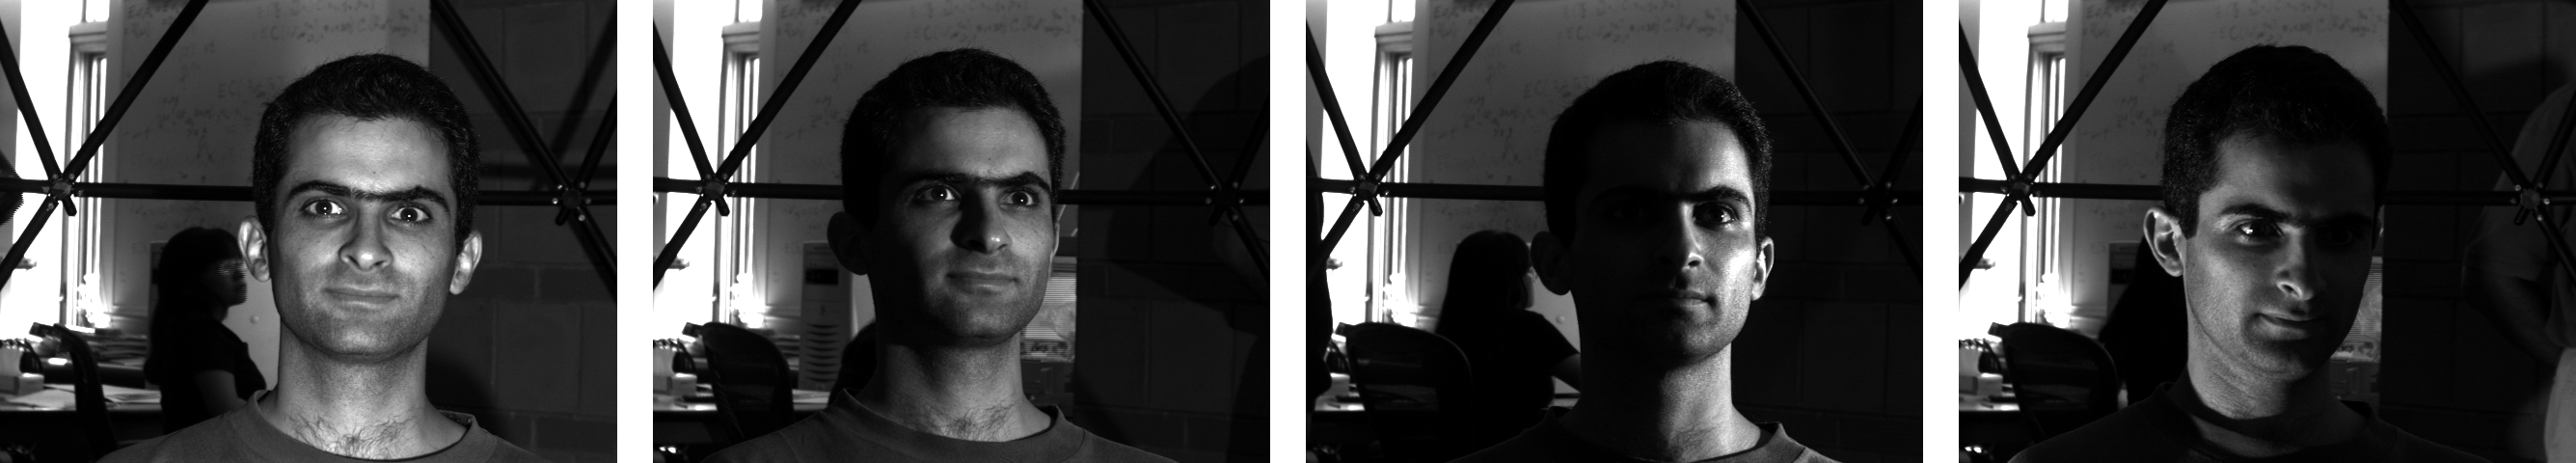
\includegraphics[scale=0.13]{figures/Dataset.png}
\end{figure}

The two methods of distortion that we use to simulate perspective effects are translation and skew. We translate images in the testing set by moving them by a certain number of pixels in the x or the y dimension, and we quantify the ``amount of translation'' by an upper bound $t$ in the total translation distance. Zero padding is used to fill in values. In order to skew each image, we create an affine transformation by rotating the image by a random angle between 0 and $2\pi$, scaling it by different factors in both dimensions, and then rotating it back by the same angle. We quantify the ``amount of skew'' as a number $p$ such that both scaling factors are in $[\frac{1}{p}, p]$. Examples of these effects can be seen in figure 2.

\begin{figure}
\caption{One sample from our data set as it is translated, skewed, and both translated and skewed.}
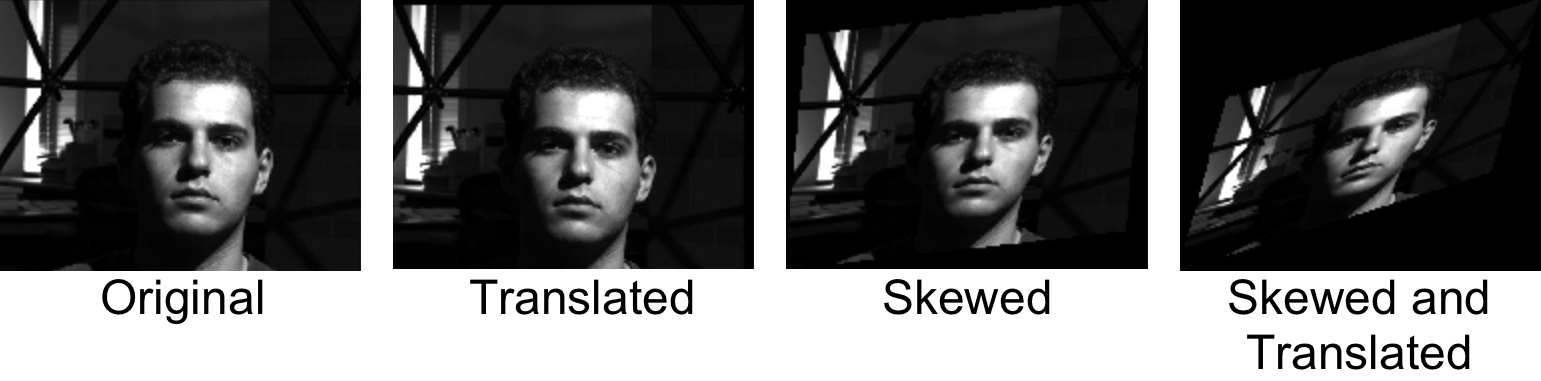
\includegraphics[scale=0.23]{figures/Distortion.png}
\end{figure}

\section{Results}

In order to train and test the model on a laptop computer, we limited our data set to only 15 classes (people), with 20 randomly selected samples from each class used for training, and 15 randomly selected samples from each class used for testing. Without any of our distortions, the model correctly classified 222 out of 225 testing set samples, or 98.7\%.
% \note{Should we mention that it consistently ran at such high percentages so it doesnt sound like we just ran it once and got something good}

We then translated each of the samples in our testing set by a random number of pixels between 0 and $n$, with $n\in\{0,5,10,...,50\}$. This yielded a sharp decrease in the number of samples which were correctly classified, as can be seen in figure 3.

\begin{figure}
\caption{Accuracy as testing set is translated by different pixel amounts}
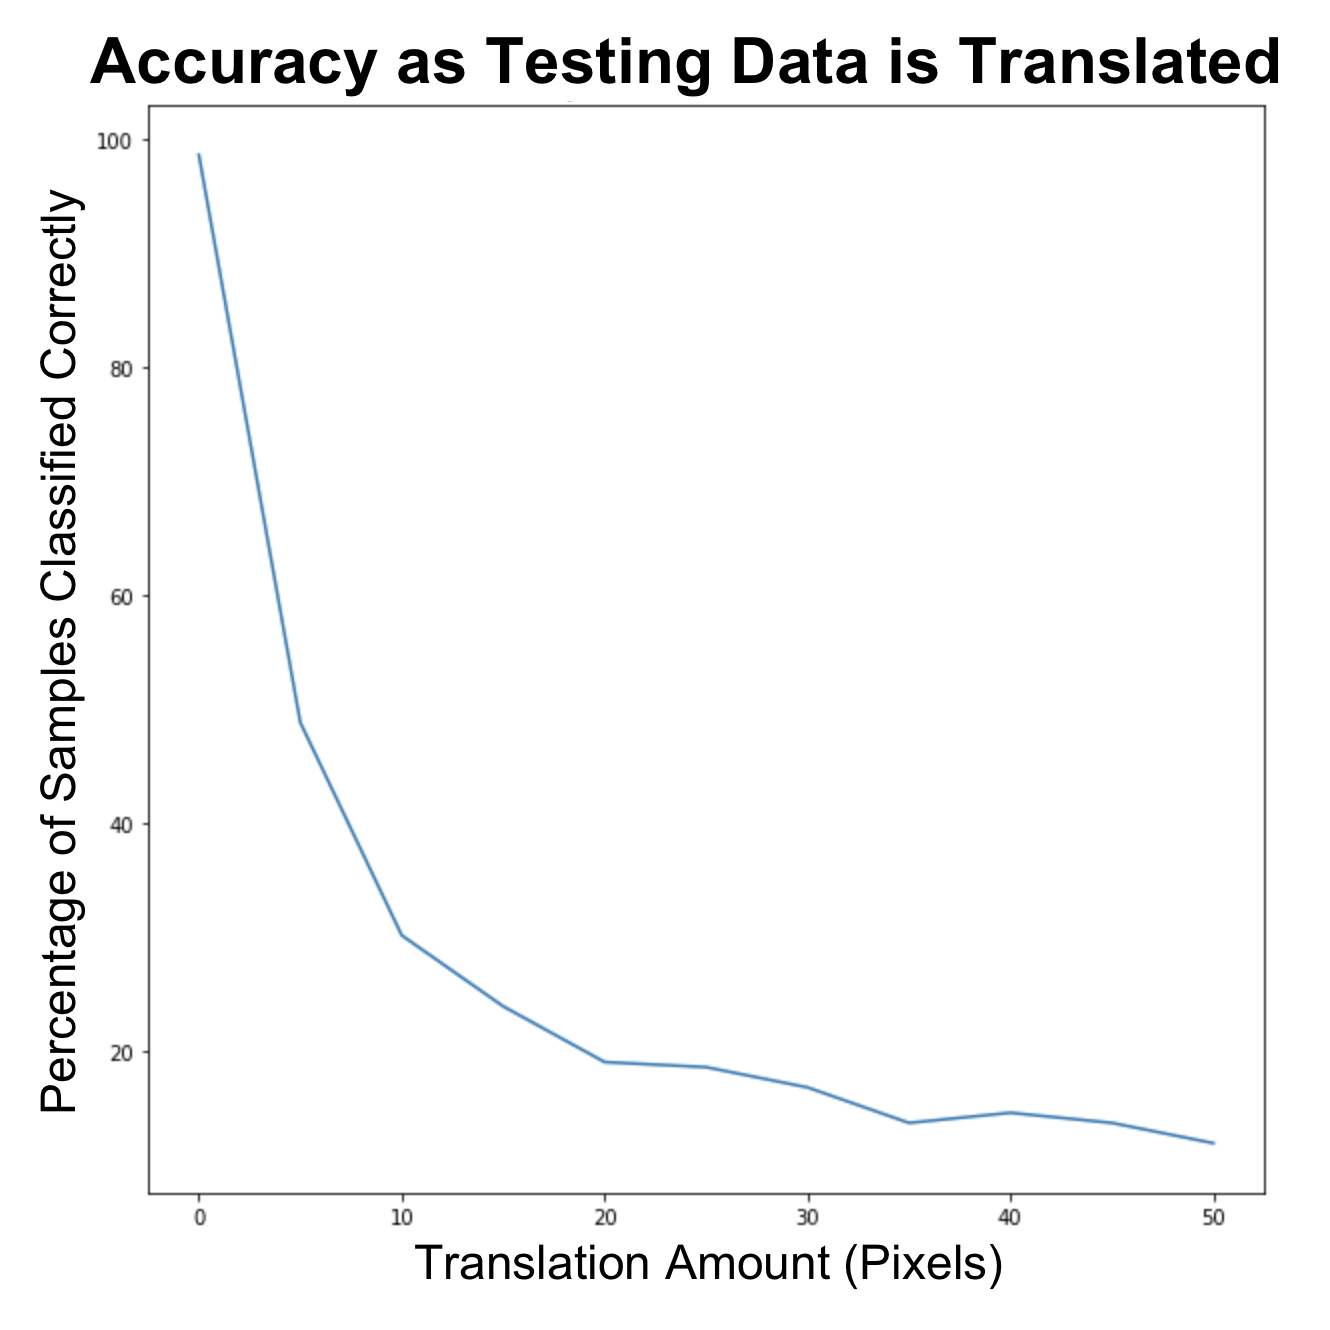
\includegraphics[scale=0.25]{figures/Translation.png}
\end{figure}

We separately simulated distortion arising from perspective effects by skewing each image. As before, we applied this skew to each of the testing set images, with the skew factor randomly assigned to a number between $1/n$ and $n$ for $n\in\{2,3,...,10\}$. We present our findings in figure 4. As with translation, there is a sharp drop-off in the algorithm's performance, however the accuracy is universally much lower. With a very high skew, the algorithm's performance approaches that of randomly assigning each image to one of the 15 classes (6.67\%).

\begin{figure}
\caption{Accuracy as testing set is skewed by different factors}
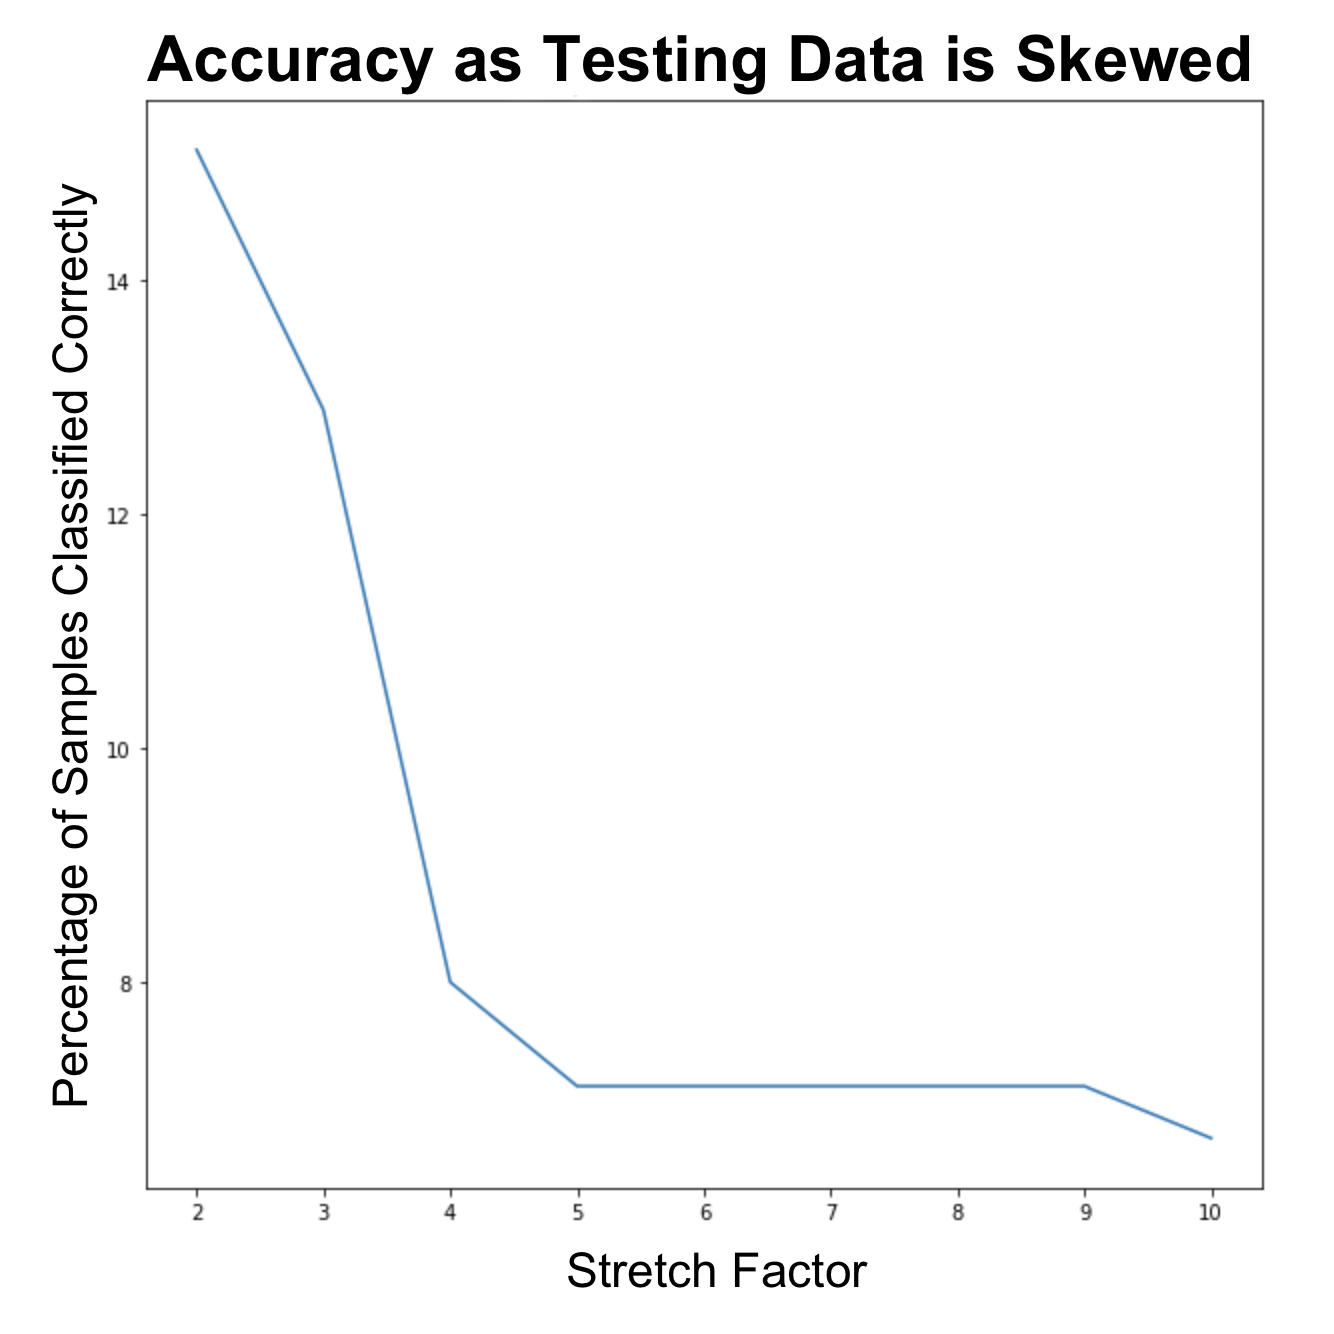
\includegraphics[scale=0.25]{figures/Skew.png}
\end{figure}

Finally, we simulated both distortion and translation by applying both the skew and the translation effects to each of the images in the testing set. For integer $n\in\{0,1,...,8\}$, we translated each image by a random number of pixels between 0 and $10+5n$ and skewed it by skew factor $2+n$. Our results, seen in figure 5, closely resemble those of skew-only distortion, however at each step, the accuracy is roughly one percentage point lower without the addition of translation.

\begin{figure}
\caption{Accuracy as testing set is skewed and translated by different factors and pixel values}
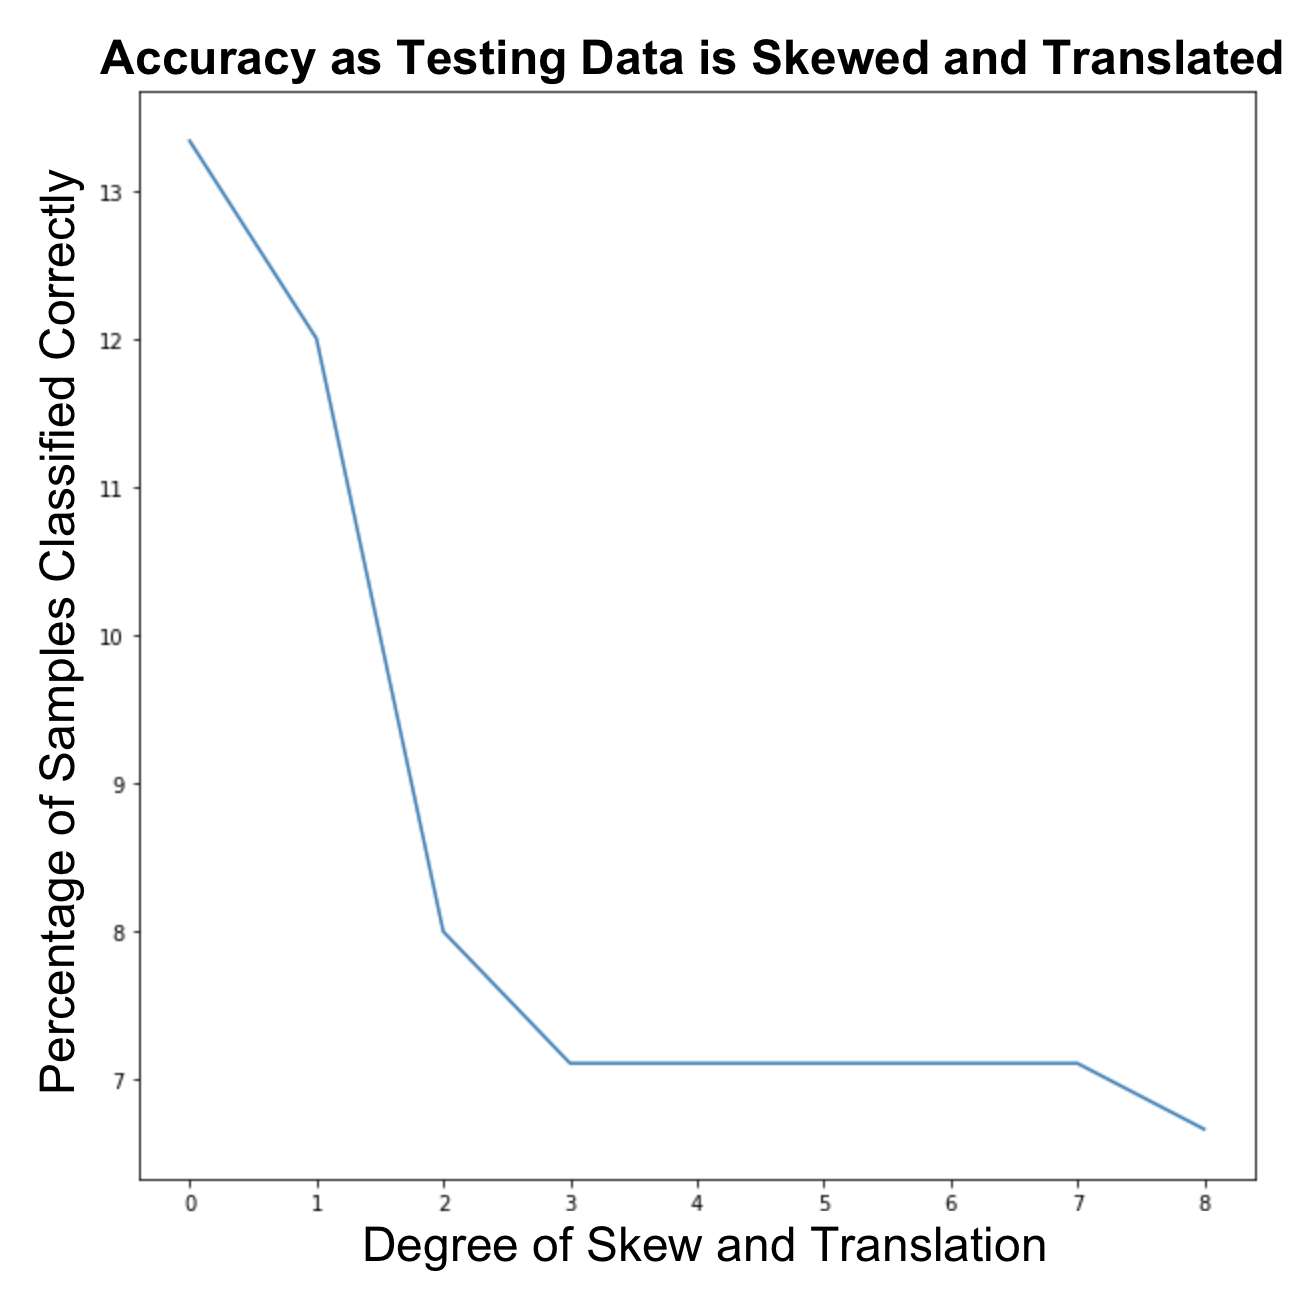
\includegraphics[scale=0.25]{figures/SkewTranslation.png}
\end{figure}

\section{Conclusion}

While we find that the algorithm performs remarkably well on our unaltered data set, as had been predicted in the original paper, this performance does not extend well to our simulated distortion effects. Under translation only, algorithm performance decreases sharply after each image is translated just a few pixels in the x or the y directions. Under simulated skew effects, the performance loss is even more drastic as accuracy quickly approaches that of random classification to one of the 15 classes. Finally, composing both skew and rotation creates nearly identical behavior with slightly worse accuracy at each step.

Looking forward, significant changes to the algorithm are needed in order to correctly identify faces under the distortion created by projecting three-dimensional perspective effects onto a two-dimensional image. Though its performance is promising on staged data sets such as The Extended Yale Database B, real world applications of facial recognition require a system that is more robust to perspective alterations.

\section{Contribution Statement}
I started a first implementation of the paper and realized that the scatter matrices were too big to compute, so going off of Dor's advice, I figured out how to use SVD to bypass computing the scatter matrix when solving the generalized eigenvalue problem necessary for the Fisher linear discriminant method. I wrote some pseudocode for FLD, which Toby then used to finish the implementation of FLD. We added the $k$ means clustering together and ran the first tests together. We went to Prof. Zickler's office hours to ask about meaningful tests to run for our extension and proposed our idea. After getting his aproval, we used my pset 2 code for homography application and I wrote the random distortion and translation generator, and generated the graph for accuracy with increasing translation. Toby then generated the graphs for random distortion and random distortion + translation. We wrote the final report together in a meeting. Throughout, we mostly worked together during meetings so we helped debug and correct errors in each other's code. We both spent the same amount of time outside of meetings working on the project. 

\section{References}
\noindent P. N. Belhumeur, J. P. Hespanha and D. J. Kriegman, "Eigenfaces vs. Fisherfaces: recognition using class specific linear projection," in IEEE Transactions on Pattern Analysis and Machine Intelligence, vol. 19, no. 7, pp. 711-720, July 1997.
\linebreak
\linebreak
The Extended Yale Face Database B, Yale. 2001. http://vision.ucsd.edu/~iskwak/ExtYaleDatabase/ExtYaleB.html.
\linebreak
\linebreak
R. Wang, “Generalized Eigenvalue Problem.” Generalized Eigenvalue Problem, Harvey Mudd College, 27 Apr. 2015, fourier.eng.hmc.edu/e161/lectures/algebra/node7.html.
\end{document}